\section{Street Network Analysis}\label{network-analysis}

Networks (graphs) represent entities as nodes (vertices) connected by links (edges). Graph-theoretic approaches to spatial problems trace back to Euler's solution to the Königsberg bridges problem in 1736 \cite{euler_solutio_1741}, with centrality methods later developed for telecommunication networks \cite{Shimbel1953} and social network analysis \cite{Wasserman1994}. Two common centrality measures are \emph{closeness} \cite{Sabidussi1966}, reflecting proximity to other nodes, and \emph{betweenness} \cite{Freeman1977}, reflecting how often a node lies on shortest paths between others. These measures rely on shortest-path algorithms, with distance defined either topologically (number of steps) or by traversal costs assigned to links (e.g., street lengths in metres).

Understanding why closeness formulations behave differently under localised analysis requires familiarity with several methodological distinctions: \emph{global} versus \emph{localised} analysis, \emph{primal} versus \emph{dual} network representations, and \emph{metric} versus \emph{geometric} distance. Each affects how centralities are computed and interpreted, and each represents a source of variation that can compromise reproducibility if not clearly documented.

\subsection{Scales of Analysis}

Network centrality methods can be applied to an entire city network (`global' analysis) or within distance-limited catchments (`localised' analysis). In global analysis, centrality magnitudes are coupled to network size: larger networks yield larger values. Different boundary definitions therefore produce different results, raising several issues:
\begin{itemize}
  \item Boundaries are difficult to define consistently across cities, particularly for large agglomerations. Network percolation \cite{Arcaute2016} offers one heuristic approach;
  \item Global analysis is subject to ``edge-effects'': centrality values diminish near boundaries because algorithms are constrained by the network extent \cite{Turner2007, van_nes_introduction_2021};
  \item Local-scale properties are masked by global characteristics, making it difficult to compare localised network properties across locations or assess local-scale impacts of design interventions \cite{Porta2009, van_nes_introduction_2021}.
\end{itemize}

These issues are addressed through ``localised'' network analysis, which uses a moving window to define catchment areas \cite{Turner2007}. As illustrated in Figure~\ref{fig:moving_window}, each node is visited in turn; all nodes within a specified distance threshold are identified and isolated as a subgraph; centrality is computed for that subgraph; the algorithm then proceeds to the next node.

\begin{figure}[htbp]
  \centering
  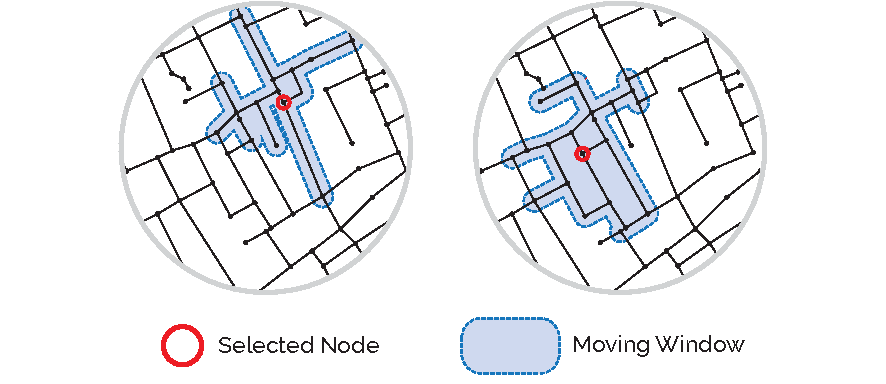
\includegraphics[width=\linewidth, keepaspectratio]{images/moving_window.pdf}
  \caption{Moving window catchment area.}\label{fig:moving_window}
\end{figure}

Localised methods confer several advantages:
\begin{itemize}
  \item Measures computed for a given distance threshold can be compared directly across locations---even across cities---because catchment extents are defined consistently;
  \item Edge-effects are substantially mitigated when the network is buffered relative to the distance threshold (e.g., a 1km buffer eliminates edge effects for 1km catchments);
  \item Different distance thresholds reveal different scales of network structure: smaller distances capture local-scale walkability; larger distances approximate global analysis without its drawbacks.
\end{itemize}

Localised analysis is now conventional practice. Throughout this paper, we use the term `localised' regardless of the distance threshold. Critically, in localised analysis the number of reachable nodes varies by origin---the condition under which different closeness formulations diverge in behaviour.

\subsection{Model Representations}\label{network-representations}

In the \emph{primal} representation, intersections are nodes and streets are links, corresponding to streets embedded in Euclidean space \cite{Porta2006a}. Space Syntax emerged around the \emph{dual} representation \cite{Hillier1984}, originally using \emph{axial lines}---uninterrupted lines of sight connecting convex spaces---where nodes represent street corridors and links represent topological steps between them. The algorithmic derivation of axial lines was debated \cite{Ratti2004, Turner2005a, Porta2006a}, but newer forms of dual representation have since become prevalent: \emph{angular segment analysis} \cite{Turner2000, Dalton2001, Turner2005a, Turner2007} derives the dual network directly from road centre-lines, with nodes at segment mid-points and links representing angular or metric distances (Figure~\ref{fig:primal_vs_dual}).

\begin{figure}[htbp]
  \centering
  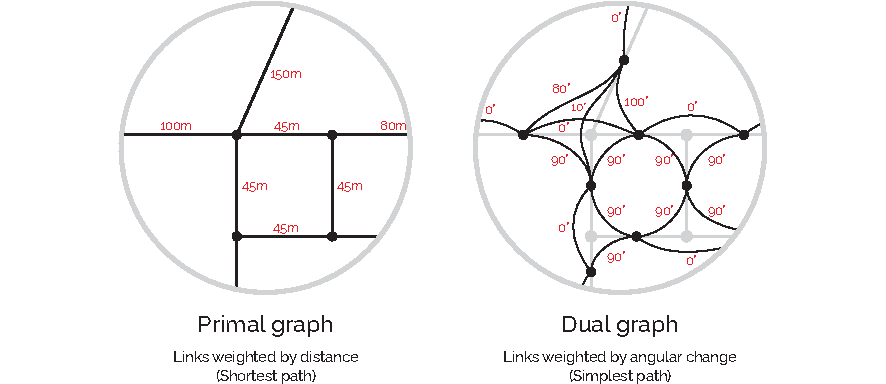
\includegraphics[width=\linewidth, keepaspectratio]{images/primal_vs_dual.pdf}
  \caption{The \emph{primal} street network representation with \emph{metric distances} (left) and a corresponding example of a dual representation (right) with \emph{geometric distances}. Note that the dual network can be used with \emph{metric distances}.}\label{fig:primal_vs_dual}
\end{figure}

While many network representations exist \cite{Marshall2018}, including those used to analyse \emph{small-world} and \emph{scale-free} properties \cite{Albert2002, Porta2006a}, contemporary street network analysis typically uses either the primal representation or its direct dual inversion, leveraging widely available street network datasets \cite{Rosvall2005, Marshall2018, Batty2004}.

\subsection{Cost Parameters}

Links can be assigned traversal costs reflecting different notions of distance. \emph{Metric distance} uses physical units (metres); \emph{geometric distance} uses angular deviation, favouring straighter routes with better lines-of-sight over convoluted ones regardless of physical length \cite{Hillier2007, Serra2019}. Geometric distance is preferred in space syntax, where route linearity is considered an important determinant of land-use patterns and urban activity \cite{Penn1998}.

Geometric distance introduces an implementation nuance: shortest-path algorithms may `bypass' sharp turns by combining adjacent smaller angles (Figure~\ref{fig:enforced_dual}). Specialised tools such as \emph{depthmapX} \cite{turner_depthmapx_2020}, \emph{Place Syntax Tool} \cite{stahle_place_2023}, and \emph{cityseer} \cite{simons_cityseer_2023} enforce directional constraints to handle this correctly; generic network packages typically do not \cite{Turner2007, banino_vector-based_2018}.

\begin{figure}[htbp]
  \centering
  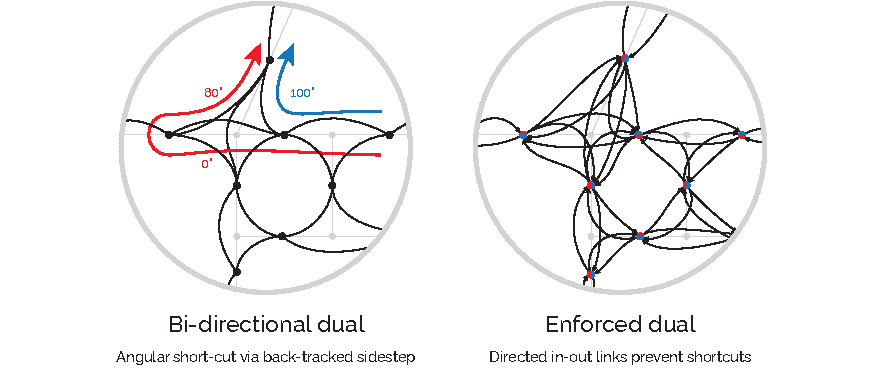
\includegraphics[width=\linewidth, keepaspectratio]{images/enforced_dual.pdf}
  \caption{Shortest angular path side-stepping.}\label{fig:enforced_dual}
\end{figure}

Metric and geometric distances are not mutually exclusive; both are valid and their interrelation is complex \cite{Barthelemy2015}. Shortest routes frequently coincide under either metric \cite{Viana2013, Omer2018}, and strong correlations between them are observed at certain distances \cite{Hillier2007, Serra2019}. Research indicates geometric distance is most relevant for vehicular travel at distances exceeding 2000m, while metric distance retains relevance for smaller-scale and non-vehicular analysis \cite{Serra2019, sharmin_meta-analysis_2018}. Note that metric distances can be computed on dual representations, geometric distances on primal ones, and multiple representations can be applied simultaneously \cite{Masucci2016}.

\subsection{Distortions Related to Topology and Geometry}

Network analysis is sensitive to topological structure. Low-quality datasets---with broken links or unnecessarily complex intersection representations---produce spurious results. A common problem is conflation of topological structure with geometric trajectories: a curved street may be represented with additional nodes to approximate its geometry, inflating centrality summations relative to a straight street of equivalent length.

Cleaned network representations that separate geometry from topology are therefore essential. Networks from sources such as OpenStreetMap typically require simplification while preserving segment geometry to ensure accurate distance and angle measurements \cite{gil_road_nodate}. In this research, the \texttt{cityseer} package facilitates these techniques \cite{simons_cityseer_2023}. Formalisation of network simplification methods is an active area of interest \cite{krenz_employing_nodate}.

A related issue is topological divergence between primal and dual representations (Figure~\ref{fig:primal_vs_dual_structure}). Even when derived from the same underlying structure, these representations yield different centrality values because the dual generates more nodes and links, particularly in complex networks. Comparative evaluation between metric measures on primal networks and geometric measures on dual networks should be avoided, as differences will reflect representation as well as the underlying network properties.

\begin{figure}[htbp]
  \centering
  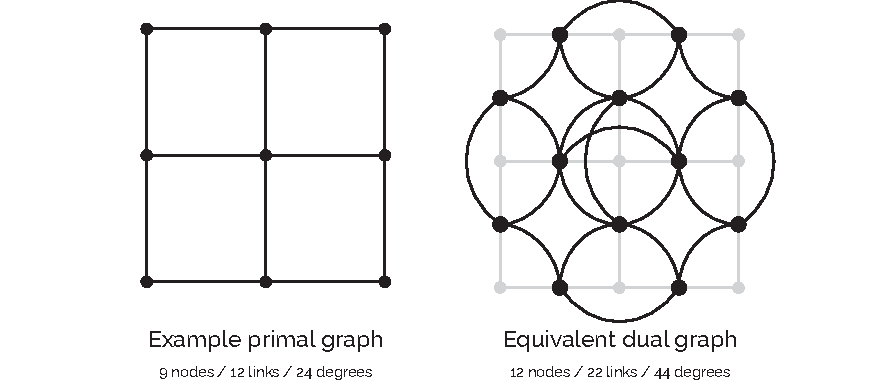
\includegraphics[width=\linewidth, keepaspectratio]{images/primal_vs_dual_structure.pdf}
  \caption{Topological divergence of primal and dual representations.}\label{fig:primal_vs_dual_structure}
\end{figure}
